\documentclass[tikz,border=2pt]{standalone}
\usepackage{amsmath}
\usepackage{amssymb}
\usepackage{pgfplots}
\pgfplotsset{compat=1.18}
\usetikzlibrary{arrows.meta}
\begin{document}
% Setup model of Ex. 6.2.6 (lambda = 3/h, lambda_r = 0.5/h, E[S_0] = 1/4 h, V[S_0] = 1/16, E[R] = 2 h, V[R] = 1, C_a^2 = 1):
% red-job sojourn E[J_r](B) = (B-1) + E[W_B] + 2 + (B+1)/8, with E[W_B] from Sakasegawa (c = 1); B_m = 24, E[J_r](30) = 40.76 h.
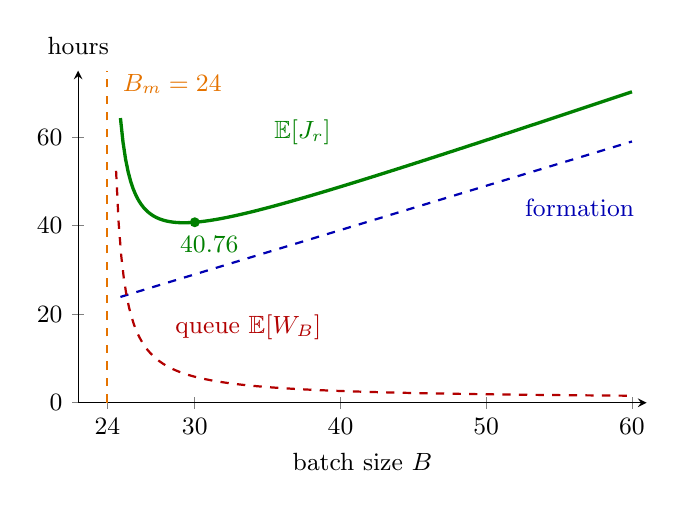
\begin{tikzpicture}[font=\small, >={Latex[length=2mm]}]
  \begin{axis}[
    axis lines=left, xmin=22, xmax=61, ymin=0, ymax=75,
    xtick={24,30,40,50,60}, ytick={0,20,40,60},
    xlabel={batch size $B$}, ylabel={hours},
    ylabel style={rotate=-90, anchor=south, at={(axis description cs:0,1.02)}},
    samples=200, width=8.8cm, height=5.8cm, clip=false]
    % total sojourn time of a red job
    \addplot[green!50!black, very thick, domain=24.9:60, restrict y to domain=0:75]
      {(x-1) + ((1/x + (1+x/16)/(2+x/4)^2)/2*(0.75+6/x)/(1-(0.75+6/x))*(2+x/4)) + 2 + (x+1)/8};
    % batch formation time (B-1)/(2 lambda_r)
    \addplot[blue!70!black, thick, dashed, domain=24.9:60] {x-1};
    % batch time in queue (Sakasegawa)
    \addplot[red!70!black, thick, dashed, domain=24.6:60, restrict y to domain=0:75]
      {(1/x + (1+x/16)/(2+x/4)^2)/2*(0.75+6/x)/(1-(0.75+6/x))*(2+x/4)};
    \draw[orange!90!black, thick, dashed] (axis cs:24,0) -- (axis cs:24,75);
    \node[orange!90!black, anchor=west] at (axis cs:24.4,72) {$B_m=24$};
    \fill[green!50!black] (axis cs:30,40.758) circle (1.8pt);
    \node[green!50!black, anchor=north] at (axis cs:31,39.8) {$40.76$};
    \node[green!50!black, anchor=south east] at (axis cs:40,56) {$\mathbb{E}[J_r]$};
    \node[blue!70!black, anchor=west] at (axis cs:52,44) {formation};
    \node[red!70!black, anchor=south west] at (axis cs:28,12) {queue $\mathbb{E}[W_B]$};
  \end{axis}
\end{tikzpicture}
\end{document}
